\section{Results}\label{results}

\subsection{Code testing}

The IIEE module being implemented, some tests were required in order to check that the code behaves accordingly. To do so, several tests were realised. The first one consisted of statistical results for the yield. To derive a statistics, the simple geometry from \ref{Theory_axy} was implemented, as well as several horizontal slices of ions. These ions were initialised at different radial distances from the cathode. Making use of Eq.(\ref{ions_energy}), their energy as they hit the electrode is known, and so is the average yield per incident ion. Recall that the yield is a function of the incident ion energy only, through the energy loss in the material,

\beq
\gamma(E) = \Lambda_{exp}\cdot \frac{dE}{dx}\Bigg|_i.\label{yield_result}
\eeq 

\noindent It is also important to note that the energy loss tables used to implement the yield curves as in Fig.(\ref{yield}) contained values for protons impinging on different materials. In order to obtain results exploitable for the TREX experiment, the yield for incident protons had to be replaced by the yield for other ions, as H$_2^{+}$ for example. Approximatively, since H$_{2}$ is a diatomic molecule formed of hydrogen atoms, which are protons when ionised, one can deduce the yield for H$_2^{+}$ cations through $dE(\tilde{E})/dx|_{H_2^{+}} \sim 2dE(\tilde{E}/2)/dx|_{H^{+}}$ \cite{Yield_H2}. Hence, Eq.(\ref{yield_result}) reads 

\beq
\gamma_{H_2^+}(\tilde{E}) = \Lambda_{exp}\cdot \frac{dE(\tilde{E})}{dx}\Bigg|_{H_2^+} =2 \Lambda_{exp}\cdot \frac{dE(\tilde{E}/2)}{dx}\Bigg|_{H^+},
\eeq  

and then 

\beq
\gamma_{H_2^+}(E) \simeq 2\cdot \gamma_{H^+}(E/2). \label{Yield_H2+}
\eeq
\noindent For all three materials, the slices of ions were initialised along the axial direction, thus enabling to show that the electron generation from the code, over the loss of ions, is independent of the axial position, as expected. Fig.(\ref{flat_slice}) shows the results for $H_2^{+}$ cations impinging on the cathode made either of $^{304}$SS, Cu or Al. The potential bias applied between the two electrodes is $\Delta \phi=20$ kV. The magnetic field is uniform, with field lines parallel to the electrodes, and $B=0.21$ T, as it is a value of the order of magnitude used in gyrotrons. The radial positions of the electrode were $r_a=0.001$ m for the cathode and $r_b=0.01$ m for the anode, and the ions were generated at $r_1 = 0.003$ m, $r_2=0.005$ m and $r_3=0.008$ m. Using the very simple equation Eq.(\ref{Yield_H2+}), the expected yield could be estimated and the comparison of the latter with the one obtained from the IIEE module is exposed in Table.(\ref{tab_stat}). 

\begin{figure}[h!]
\centering
	\includegraphics[width = 1.0 \textwidth]{Flatslice_stats.eps}
	\caption{\label{flat_slice} Plot of the number of particles over the number of time-steps. The black curve represents the number of ions, while the colored curves show the number of electrons produced in the impingement of $H_2^+$ ions over $^{304}$SS, Cu and Al.}
\end{figure}  

\noindent One notes on Fig.(\ref{flat_slice}) that the ions population curve is discontinuous. It is due to the fact that the ions are initially configured in three slices at distinct radii, as shown in Fig.(\ref{slice_config}), and together with the symmetry of the system, they reach the cathode and disappear at distinct discrete times, hence the steps. Regarding the peaked shape of the electronic population curves, they disappear few time after being generated because in this geometry, the magnetic field lines are parallel to the electrodes. Thus, of a Larmor gyration, the electrons are not moving away from the cathode, and hence, they are recaptured few after being emitted.\\

\begin{figure}[h!]
\centering
	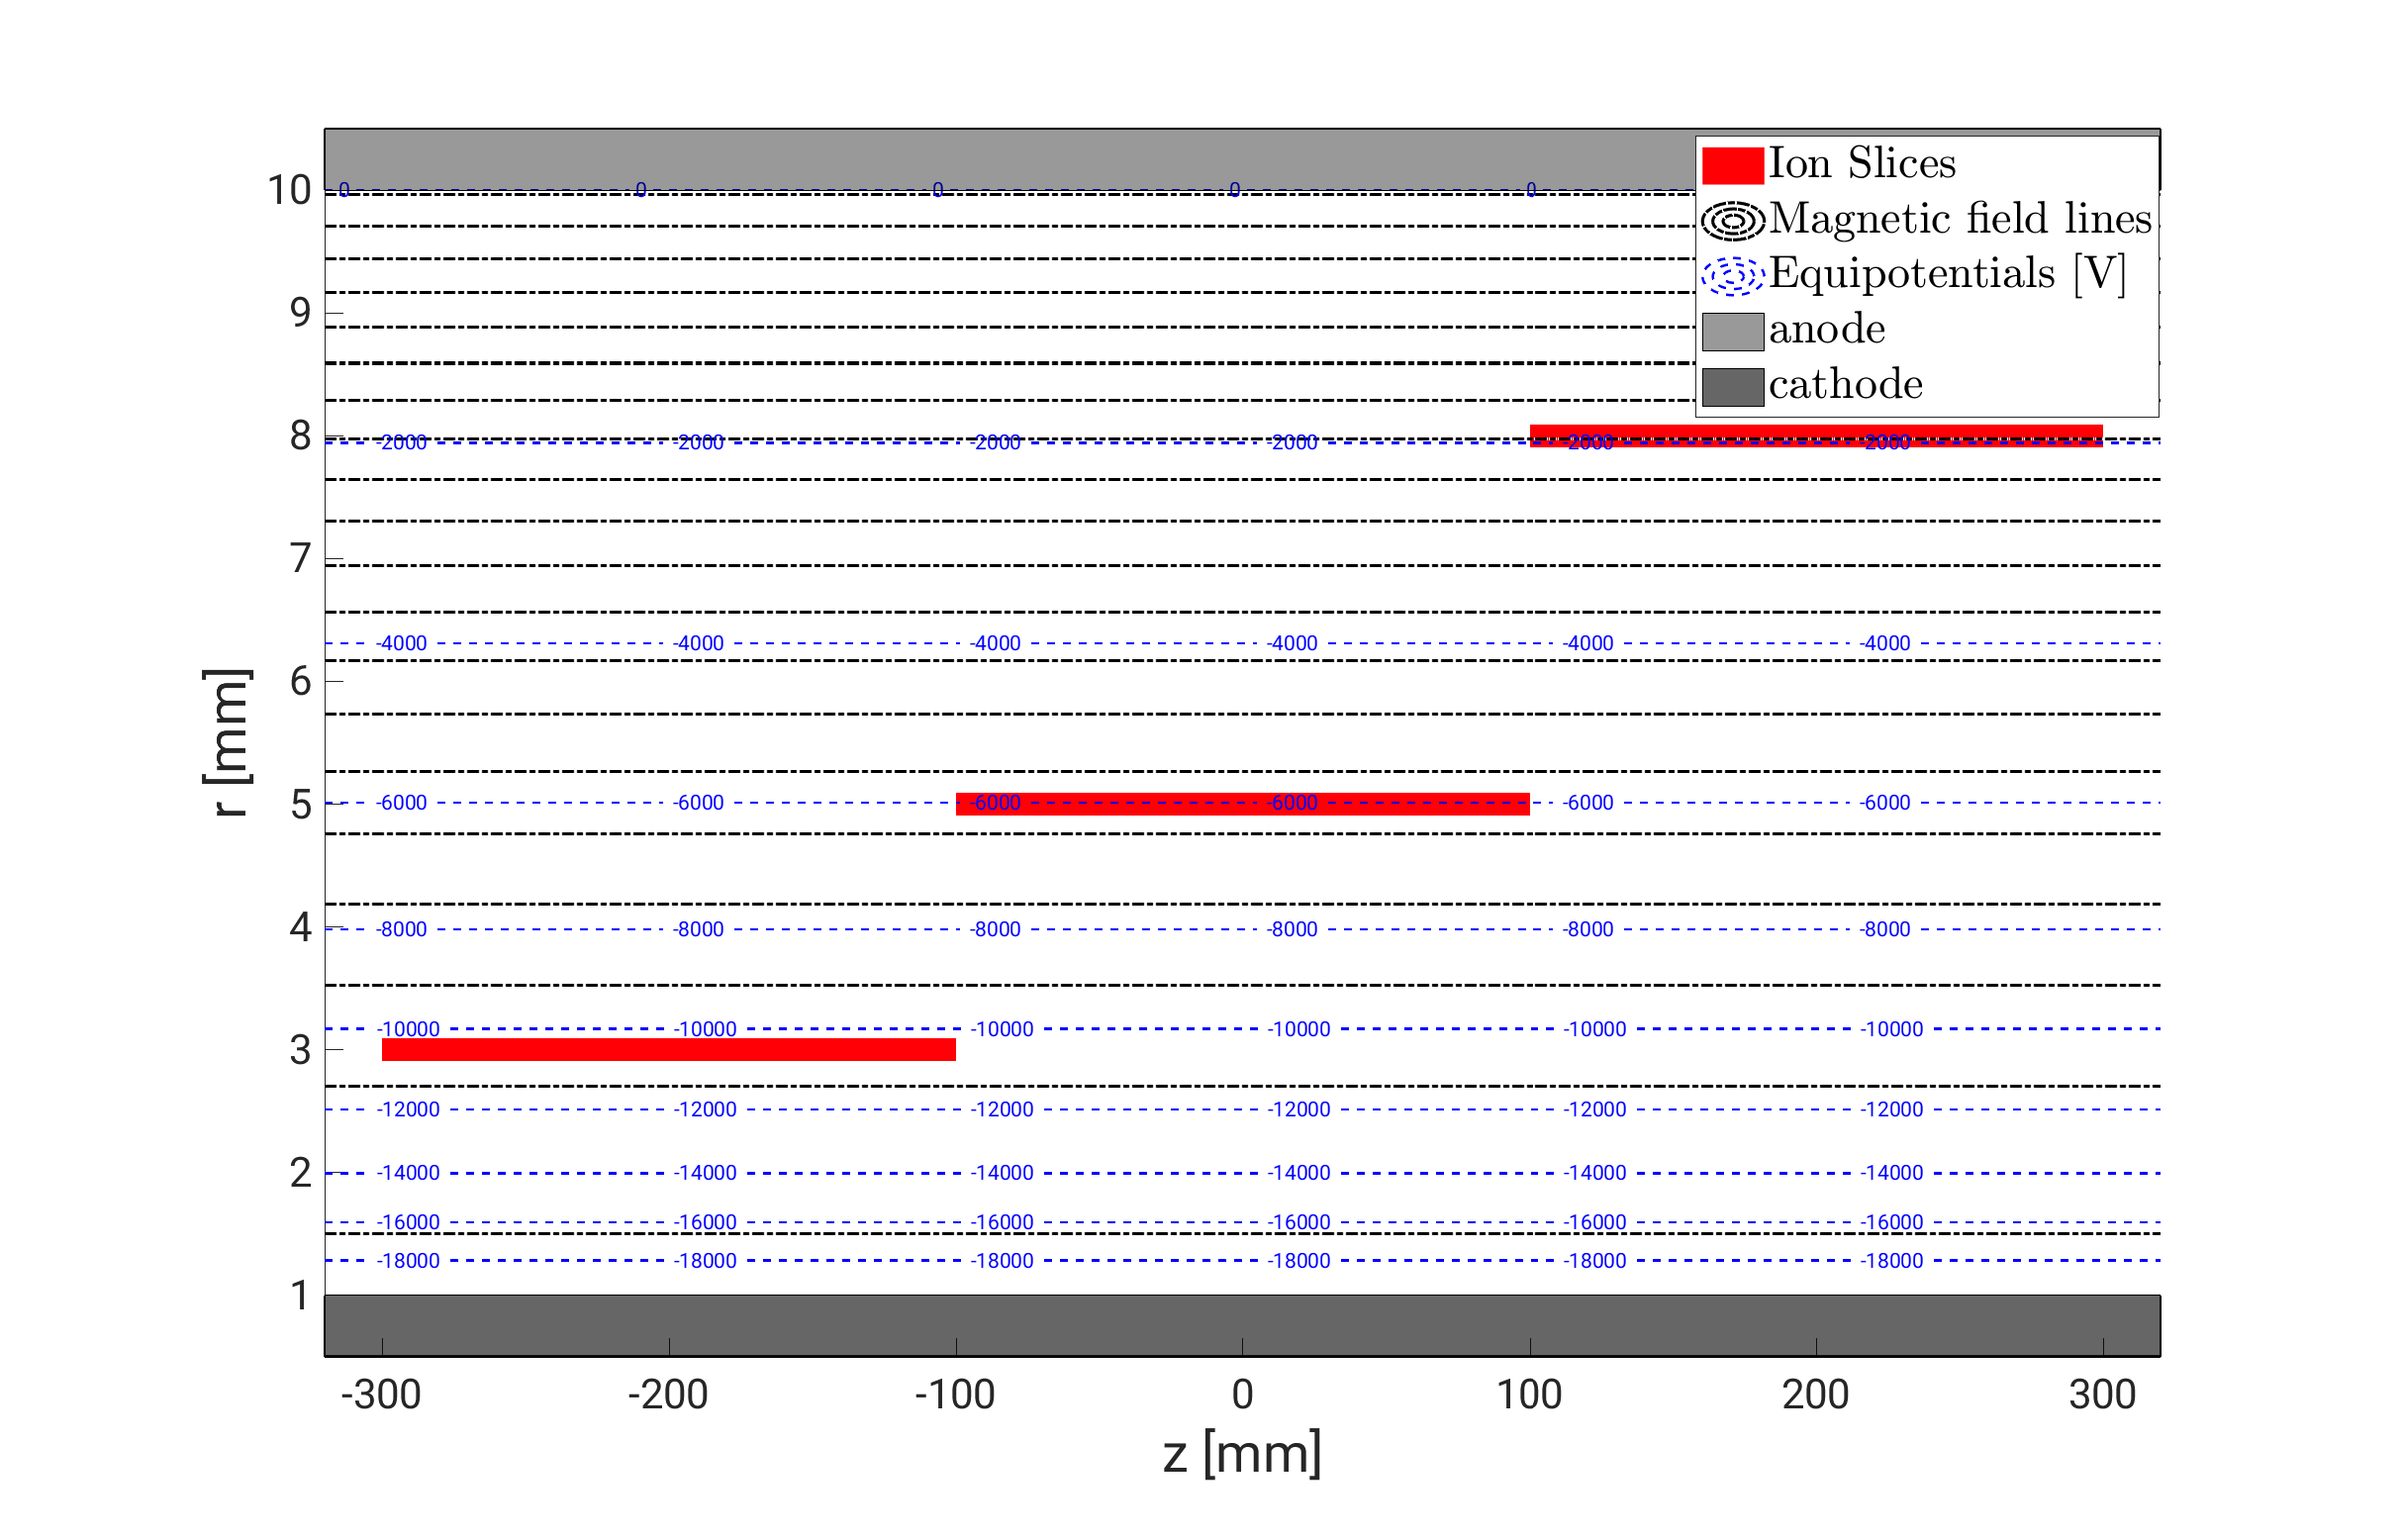
\includegraphics[width = 0.6 \textwidth]{FlatSlice_config.eps}
	\caption{\label{slice_config}  }
\end{figure}  

The statistical results presented in Table.(\ref{tab_stat}) are interesting in the sense that the theoretical model seems to have been implemented correctly. Regarding the relative errors, they are always lesser or equal to $1.6\%$, which is an acceptable value considering the fact that the model is approximative in several ways. Indeed, the yield conversion from $H^+$ to $H_2^{+}$ exposed in Eq.(\ref{Yield_H2+}) is an approximation. The fact that the yield in the potential emission region was constant (see Eq.(\ref{pot_em})), and that we linearly interpolated this constant value to the bottom of the kinetic emission model, constitutes one more source of approximation. However, this description is sufficient for a simple estimate of the influence of IIEE on electron clouds formation and behavior. Indeed, the yield being of the order of $\sim 1-2$, the approximations made should not influence or disturb greatly the expected results, in terms of electronic densities for example. \\

\begin{table}[h]
  \centering
  \renewcommand{\arraystretch}{1.2}
  \begin{tabular}{|p{5cm}|c|c|c|c|cl}
    \hline
    \center{\textbf{$^{304}$SS}}& $E_1$ & $E_2$ & $E_3$\\
     \hline
    $\gamma_{th}$ & 1.311  & 1.623 & 1.870  \\ \hline
    $\gamma_{iiee}$ & 1.299 & 1.627 & 1.891   \\ \hline
    $\epsilon_{rel}$ & 0.9\% & 0.2\% & 1.1\%  \\ \hline
     %----------------------------------------------------------------
    \center{\textbf{Cu}} & $E_1$ & $E_2$ & $E_3$ \\
     \hline
    $\gamma_{th}$ & 1.237 & 1.522 & 1.746   \\ \hline
    $\gamma_{iiee}$ & 1.229 & 1.518 & 1.760  \\ \hline
    $\epsilon_{rel}$ & 0.6\% & 0.3\% & 0.8\%  \\ \hline
     %----------------------------------------------------------------
     \center{\textbf{Al}}& $E_1$ & $E_2$ & $E_3$ \\
     \hline
    $\gamma_{th}$ & 0.920 & 1.133 & 1.297  \\ \hline
    $\gamma_{iiee}$ & 0.910 & 1.115 & 1.293   \\ \hline
    $\epsilon_{rel}$ & 1.0\% & 1.6\% & 0.3\%  \\ \hline
  \end{tabular}\caption{Yield statistics for H$_2^{+}$ ions impinging on the three materials}\label{tab_stat}
\end{table}

The last phase of the module testing was to determine wether or not some of the electrons generated by ions colliding with the electrodes would be kept in the simulation domain, or if no matter the geometry, they would be lost, as on Fig.(\ref{flat_slice}). To do so, an initial non-zero ion density was implemented in a region that was known to trap electrons, in a geometry where the cathode has half an ellipse dug inside it, as shown in Fig.(\ref{config_trapped}) - Left. This is one of the geometry planned to be mounted in the TREX experiment. No electron cloud was present at the time, so the potential well naturally present due to the topology of the $\mathbf{E}$ and $\mathbf{B}$ fields was not affected by the presence of an electron cloud. All the electrons produced at the electrode by IIEE were tracked down in a specific species in the code, so they would not be mixed up with the other electrons, coming from ionisations of the RNG. The right plot of Fig.(\ref{config_trapped}) shows the orbits of two among all the electrons that have not left the simulation domain. One notes that they were trapped in the potential well, bouncing at its axial limits, while they were drifting azimuthally over several full poloidal periods. The radial width of the orbit is defined by the Larmor radius. With this information in hand, it appears that ion induced electron emissions could produce interesting results regarding the formation of clouds. For example, the formation time could be influenced, the maximum density too. This will be treated in the next subsection.\\

\begin{figure}[h!]
\centering
	\includegraphics[width = 1.0 \textwidth]{config_trapped_rect.jpg}
	\caption{\label{config_trapped} }
\end{figure}  

\subsection{Cloud formation}

Now, let us deal with results concerning the clouds formation and dynamic, with and without taking account for IIEE. In first considerations, two particular TREX geometries have been implemented. Let us start with results in the \emph{slanted} geometry, that is with a prominent half-ellipse coming out of the anode, as in Fig.({\ref{TREX_schematics}}).\\

\textbf{TREX \emph{slanted} geometry}\\

Several characteristics are of interest in this case. As mentioned before, the characteristic time of cloud formation might be affected by the IIEE. The peak cloud density could also be increased. It can be interesting to look up the currents present at the boundaries too. Indeed, a strong electric current is as much as the source will not have to supply. To obtain these informations, two situations are considered. The geometry is the same for both, that is with the ellipse protruding from the anode. The anode is grounded, and the cathode is at $\Phi = -20$ kV. The magnetic field intensity is of about $B = 1.15$ T on the high field side (low $z$), and decreases down to $B=0.15$ T on the low field side (high $z$). The magnetic field topology and the initial electronic configuration are shown together in Fig.(\ref{Config_mag_Slanted}). Since the bottom of the ellipse is know to be a trapping region, a rectangle distribution of electrons is initialised below it, in order to act as a source of ionisation, to produce the ions by collisions with the RNG. Now two cases are to be distinguished: the case with and the case without IIEE.\\

\begin{figure}[h!]
\centering
	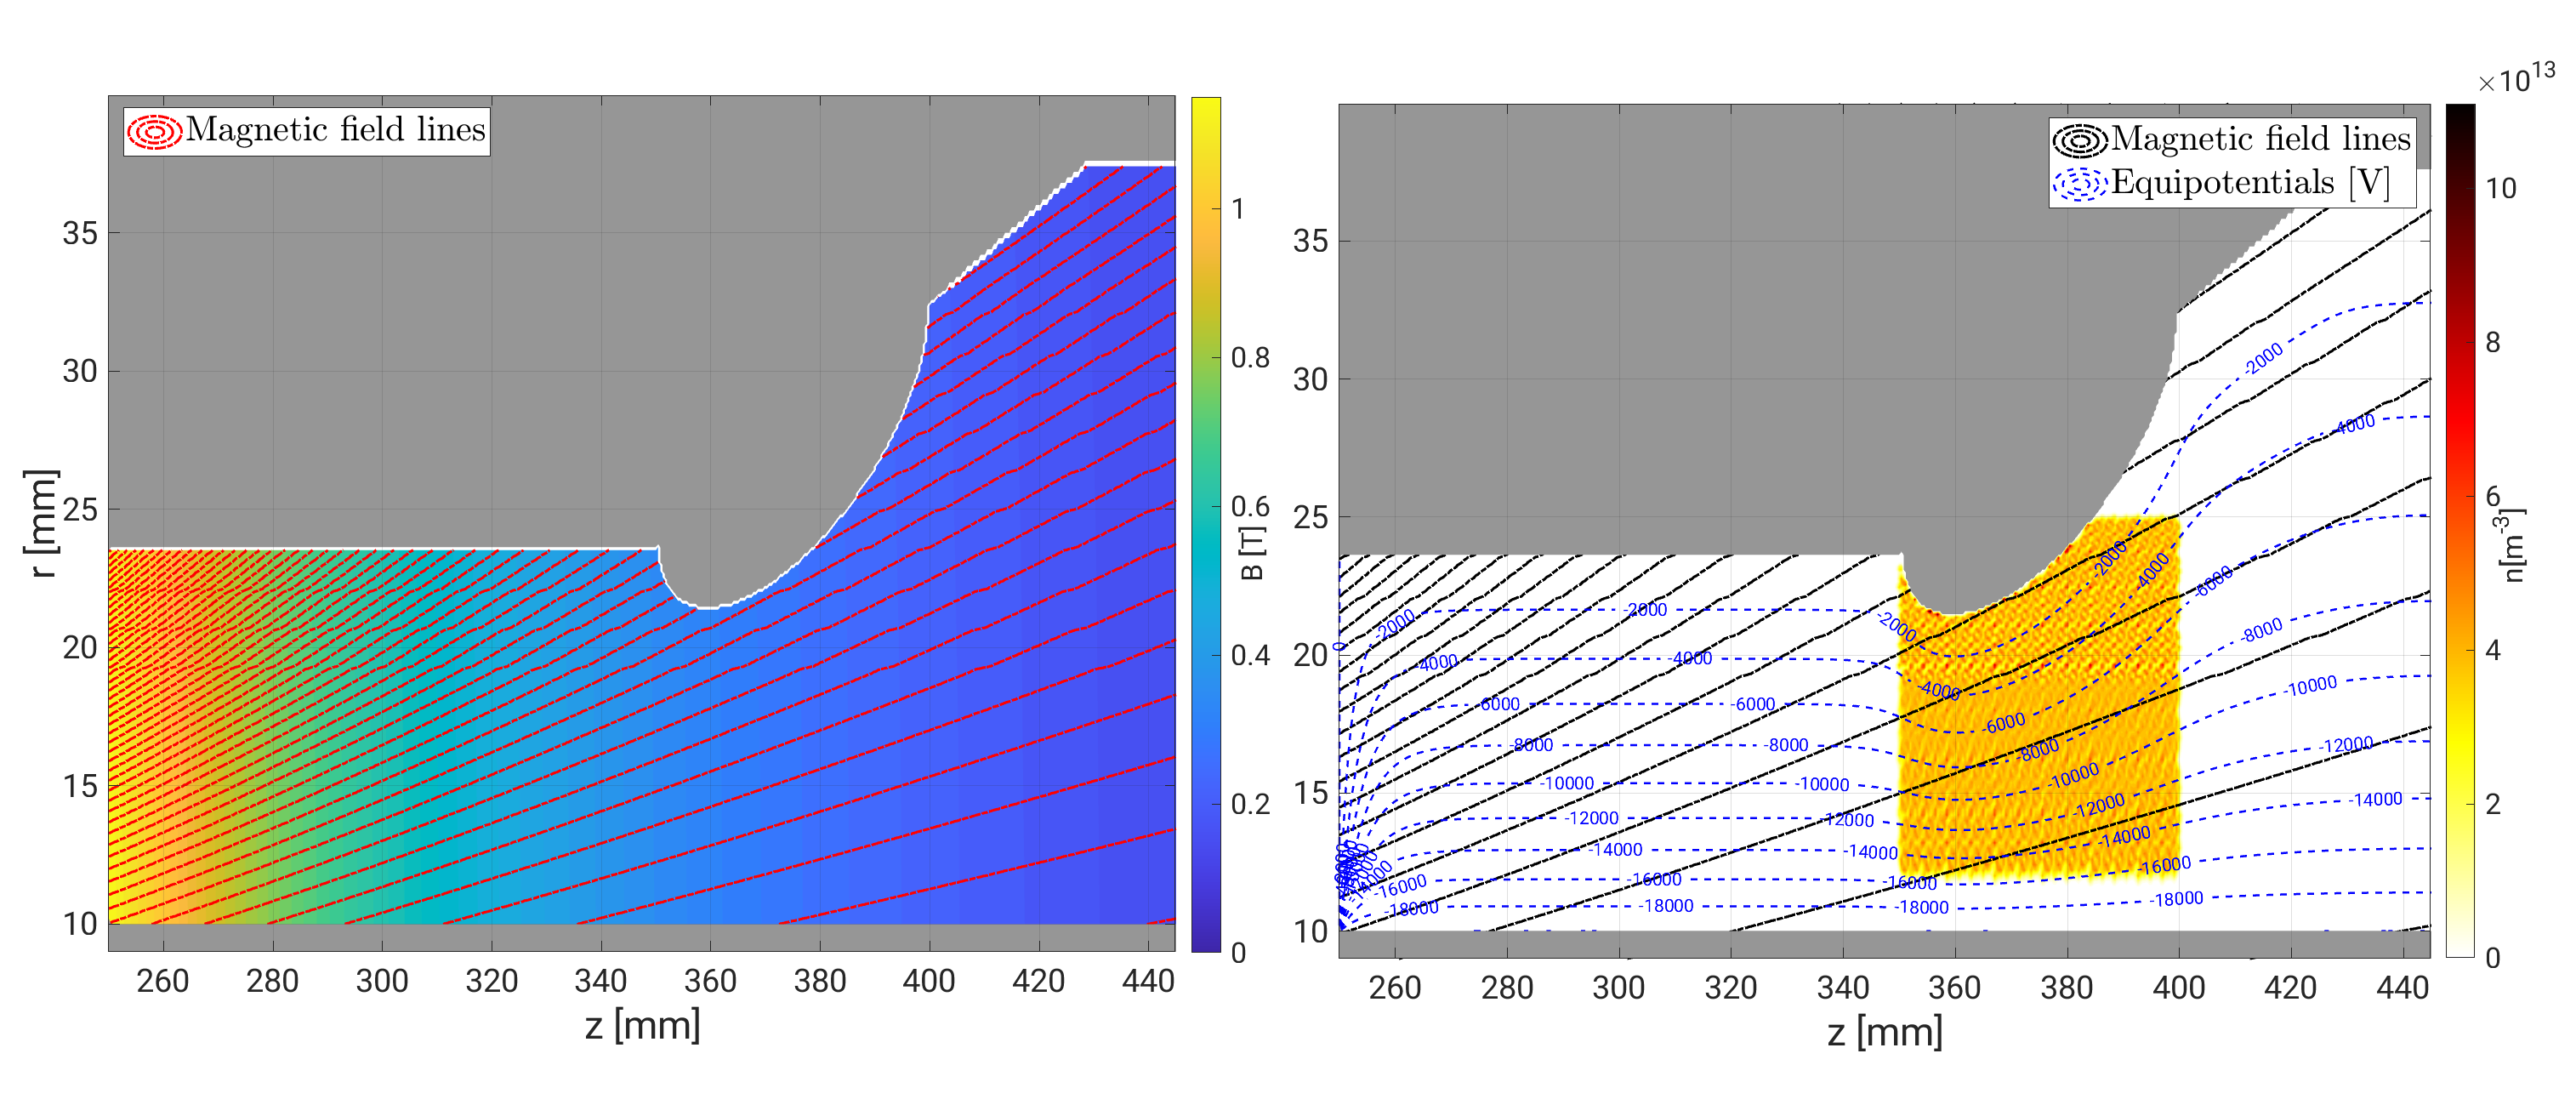
\includegraphics[width = 1.0 \textwidth]{Config_H2Slanted.eps}
	\caption{\label{Config_mag_Slanted} }
\end{figure}  


Let us first compare how fast the steady state is reached in both situations. Recall that the steady-state is characterized by the ions loss equal to the electrons loss. Hence, this is supposed to imply that the ionic current and the electronic current are equal and constant over time. Regarding the number of particles, it is supposed to reach a maximum and stagnate. The time required to reach this maximum corresponds to the cloud formation time. Plotting the total electronic charge over time can be a great indicator of the state of formation of the cloud. It can also enable to compare the formation in the two situations, where IIEE are considered and not. \\

\begin{figure}[h!]
\centering
	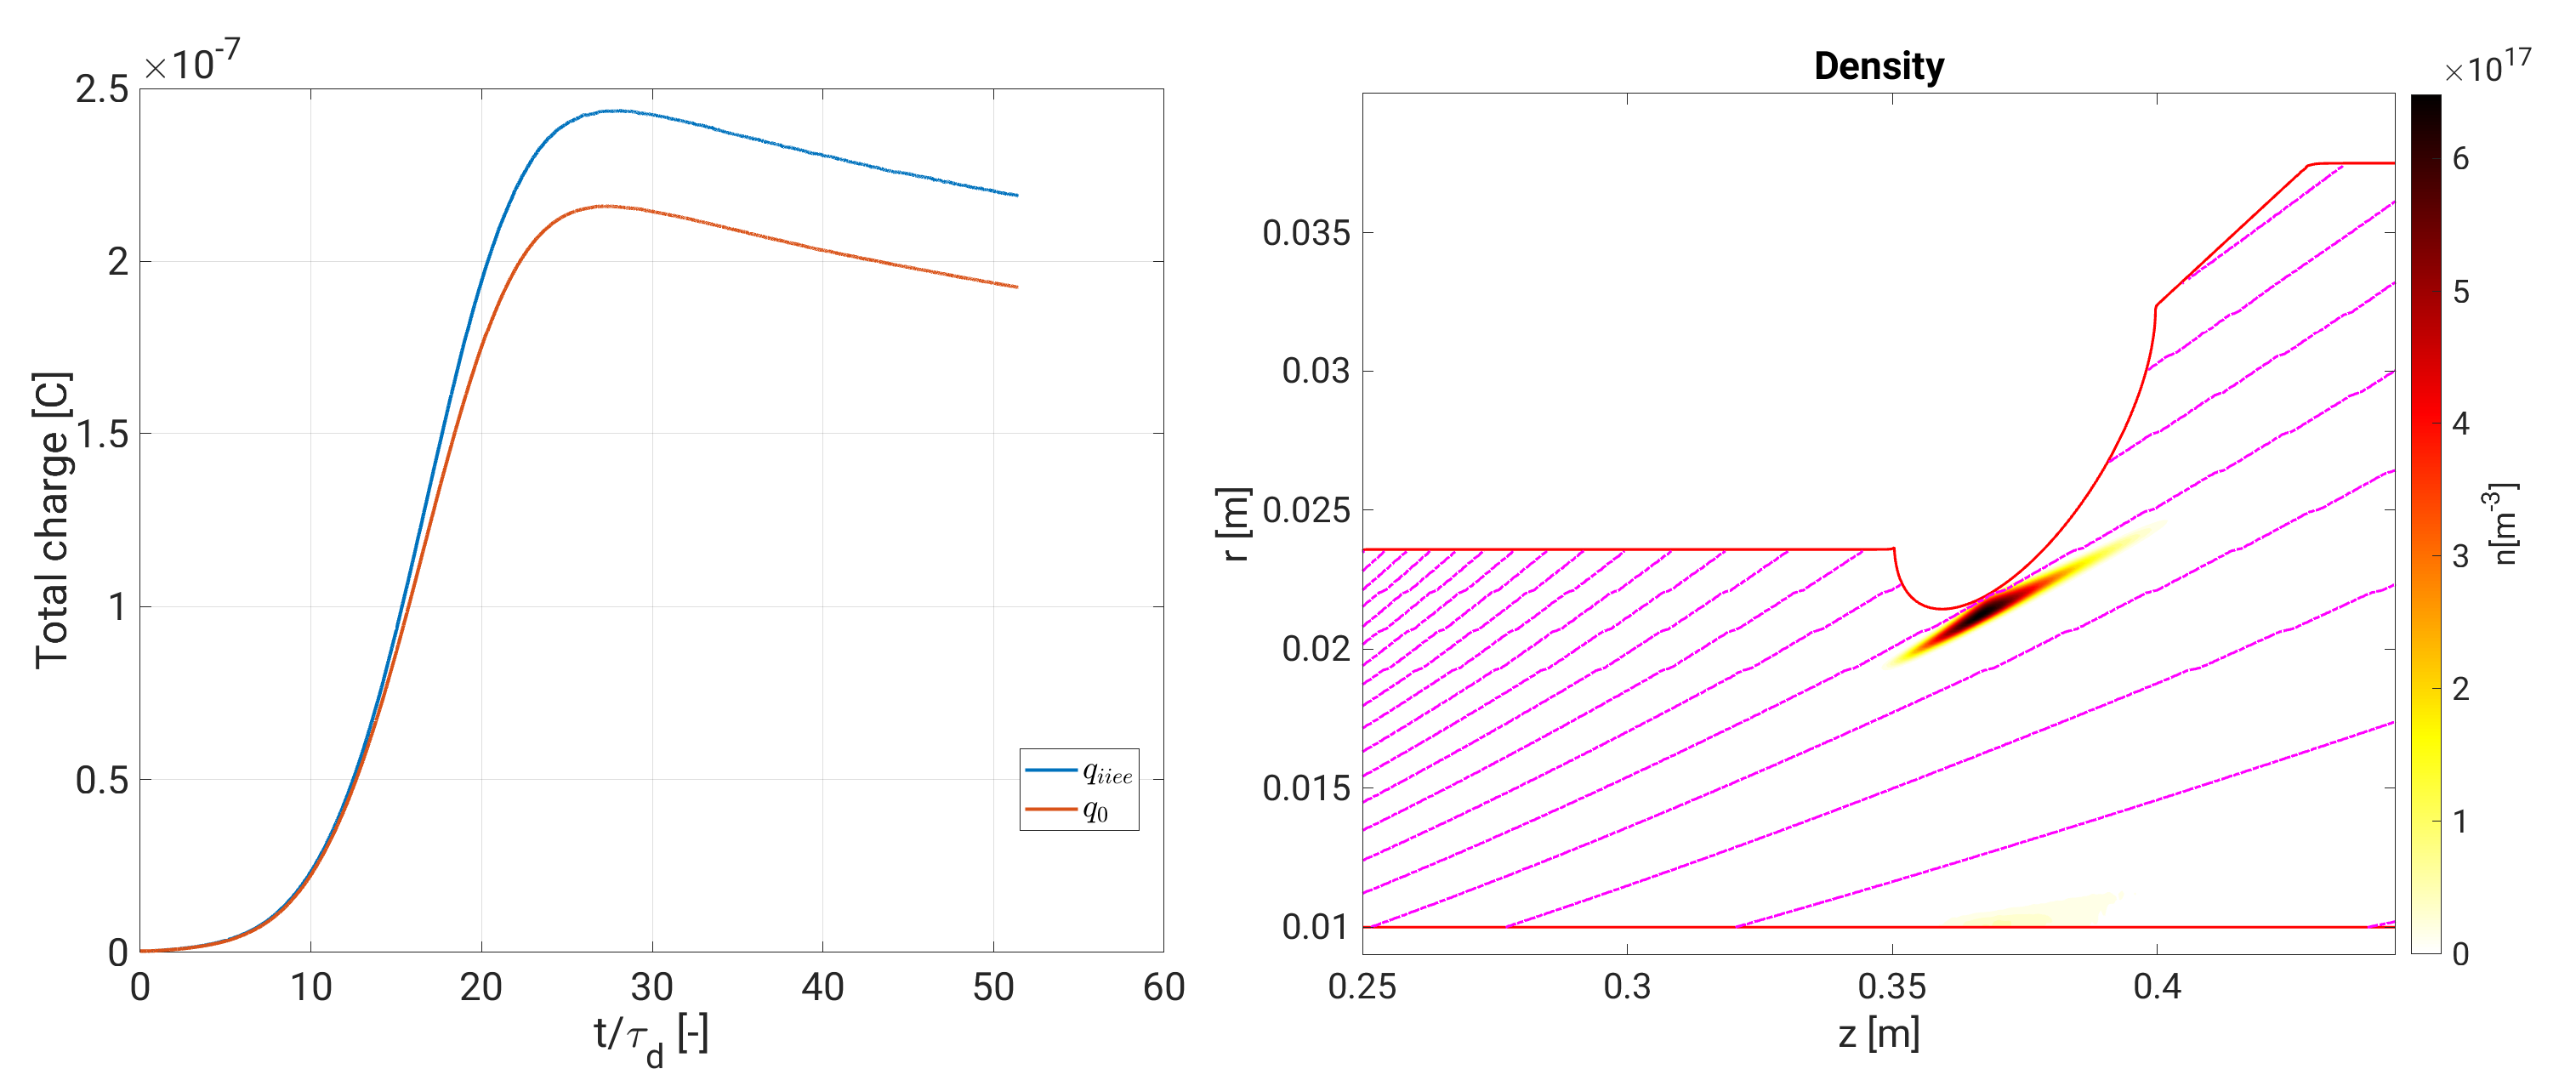
\includegraphics[width = 1.0 \textwidth]{elec_density_current.eps}
	\caption{\label{elec_density_current} }
\end{figure}  

On the left part of Fig.(\ref{elec_density_current}), the absolute value of the total electronic charge in the domain is represented over time, the time being normalised by the collision time, to remove the pressure dependency. The blue curve represents the charge when the ion induced emissions are taken into account. As expected the charge is higher, since more electrons have been produced. Note that this information alone is not sufficient to determine wether the total charge is higher because more electrons have accumulated in the cloud, or if they are present elsewhere in the domain. This is why the electron density is plotted in steady state, on the right plot of Fig.(\ref{elec_density_current}). Since both clouds, with and without IIEE had the exam same density and shape, only the situation with IIEE has been shown, for the sake of space. Note that the density of electrons coming out of the cathode, under the ellipse is non negligible since it is of about the same, or one less, order of magnitude as the cloud density (see colorbar). It is clear that these electrons, due to their Larmor motion along field lines, cannot reach the cloud and be trapped too. They will simply leave the domain axially, and contribute to a source of axial current. Now, one question arises: what is the order of magnitude of this ion-induced electronic current ? 

\newpage
\textbf{TREX \emph{extrude} geometry}\\



\subsection{Further implementation}